\chapter{Evaluación experimental}
\label{capitulo3}
\lhead{Capítulo 3. \emph{Evaluación experimental}}

\section{Diseño experimental}

En este capítulo se describe todas las decisiones tomadas con respecto a la experimentación; esto incluye los parámetros usados para la entonación, las particiones hechas en la validación cruzada y la estratificación, el diseño de los experimentos combinando las heurísticas con las metaheurísticas y finalmente se presentan los resultados de cada prueba realizada. 

Lo primero que se hace es entonar los algoritmos evolutivos para que devuelvan el mejor valor posible al probarse con los conjuntos de datos expuestos en la sección 2.4. Para lograr la entonación, se usa \emph{irace}, expuesto en la sección 2.6, con los parámetros de la tabla \ref{irace-param}. Se consigue una configuración de parámetros para los problemas pequeños, medianos y grandes respectivamente.

\begin{table}[]
\centering
\begin{tabular}{l c}
\hline
Parámetros & irace \\
\hline
\hline
Iteraciones                                 &  1000, 400 y 100\\
Número decimales significativos             &    4            \\
Prueba estadística                          &  t-test         \\
Nivel de significancia para prueba estadística  &  0.05           \\
Frecuencia de la prueba estadística         &    1 iteración  \\
Número de configuraciones élites            &  automática     \\
Reinicialización por convergencia prematura &     Sí          \\
Modo elitista                               &     Sí          \\

\hline
\end{tabular}
\caption{Parámetros usados para \emph{irace}}
\label{irace-param}
\end{table}

Los parámetros a entonar son: número de iteraciones, cardinalidad de la población, probabilidad de cruce, probabilidad de mutación y número del torneo. Los rangos válidos para cada parámetro se presentan en la tabla \ref{rangos}. La elección de los rangos se hace en base a los trabajos \cite{de2004reduccion,de2004reduccion,garcia2012prototype,garcia2008memetic,talbi2009metaheuristics}. Los resultados de la entonación se presentan en las tablas \ref{param-peq}, \ref{param-med} y \ref{param-grande}.

\begin{table}[]
\centering
\begin{tabular}{l c c}
\hline
Parámetros & Tipo de dato & Rangos \\
\hline
\hline

Población                & entero           &  [10,150]       \\
Probabilidad de cruce    & real             &  [0,1]          \\
Probabilidad de mutación & real             &  [0,0.01]      \\
Número del torneo        & entero           &  [1,10]         \\  

\hline
\end{tabular}
\caption{Rangos usados para los parámetros en la entonación}
\label{rangos}
\end{table}

\begin{table}[]
\centering
\begin{tabular}{l c c c c}
\hline
\multirow{2}{*}{\textsc{Parámetros}}
	& \multicolumn{4}{c}{\textsc{Algoritmos}} \\
	& GGA & SGA & MA & CHC \\
\hline
\hline
Iteraciones             &  1000    &  1000    &  1000      &  1000 \\
Población               &    70    &    90    &    21      &    33 \\
Prob. de Cruce          &   0.4837 &   0.9848 &     0.9496 &     - \\
Prob. de Mutación       &   0.0001 &  0.0057  &     0.0071 &     - \\
Número del torneo       &   -      &    3     &     1      &     - \\
\hline
\end{tabular}
\caption{Parámetros usados para los conjuntos pequeños}
\label{param-peq}
\end{table}


\begin{table}[]
\centering
\begin{tabular}{l c c c c}
\hline
\multirow{2}{*}{\textsc{Parámetros}}
	& \multicolumn{4}{c}{\textsc{Algoritmos}} \\
	& GGA & SGA & MA & CHC \\
\hline
\hline
Iteraciones             &  1000    &  1000    &  1000      &  1000 \\
Población               &    88    &    132   &    32      &    27 \\
Prob. de Cruce          &   0.5779 &   0.9859 &     0.9549 &     - \\
Prob. de Mutación       &   0.0001 &  0.0001  &     0.0004 &     - \\
Número del torneo       &   -      &    1     &     3      &     - \\
\hline
\end{tabular}
\caption{Parámetros usados para los conjuntos medianos}
\label{param-med}
\end{table}

\begin{table}[]
\centering
\begin{tabular}{l c c c c}
\hline
\multirow{2}{*}{\textsc{Parámetros}}
	& \multicolumn{4}{c}{\textsc{Algoritmos}} \\
	& GGA & SGA & MA & CHC \\
\hline
\hline
Iteraciones             &  1000    &  1000    &  1000      &  1000 \\
Población               &    102   &    122   &    35      &    37 \\
Prob. de Cruce          &   0.5158 &   0.9554 &     0.9698 &     - \\
Prob. de Mutación       &   0.0001 &  0.0078  &     0.0049 &     - \\
Número del torneo       &   -      &    7     &     3      &     - \\
\hline
\end{tabular}
\caption{Parámetros usados para los conjuntos grandes}
\label{param-grande}
\end{table}

Para la validación cruzada se usa k = 10 y se repite cada prueba 3 veces basándose en el trabajo de \emph{Cano, J.} en \cite{de2004reduccion}. Este esquema de validación cruzada se aplica a los conjuntos de tamaño pequeño como lo hacen en \cite{de2004reduccion}. Para la estratificación se adopta k = 10 para los conjuntos medianos y k = 50 para los conjuntos grandes, tal y como se determinan en \cite{cano2005stratification}, cuya idea es hacer que el algoritmo de PS no trabaje con más de 2000 instancias por estrato para reducir la cantidad a un conjunto de tamaño pequeño según la clasificación anteriormente expuesta. Además, al igual que en la validación cruzada, las metaheurísticas utilizadas son estocásticas y por lo tanto, cada una de las k pruebas realizadas se repite 3 veces, regresando el promedio de todas las pruebas realizadas como resultado.

Una vez obtenido los distintos parámetros para cada metaheurística, se procede con el experimento principal, el cual consta de utilizar los conjuntos $S$ obtenidos por CNN, ENN y RSS como base para inicializar la población de las metaheurísticas GGA, SSGA, MA y CHC.

Se elige utilizar CNN, ENN, y RSS porque son de las heurísticas más rápidas en ejecución según el trabajo de \emph{Salvador, G. et al.} en \cite{garcia2012prototype} y por el tipo de instancias que eligen: la primera heurística elige los puntos bordes mientras que descarta los internos bajo la idea de que los puntos bordes son los que realmente establecen los límites de decisión entre clases; ENN por su parte, elige los puntos internos y se deshace de los puntos bordes con la premisa de que los puntos bordes sólo agregan ruido al conjunto y por lo tanto hay que eliminarlos; por último RSS es un híbrido que preserva algunos puntos bordes y algunos internos manteniendo una distancia uniforme entre los mismos. En la figura \ref{heu} se puede apreciar la selección de puntos realizadas por cada heurística sobre el conjunto banana.

\begin{figure}[]

	\centering
	\subfigure[Banana]{\label{fig:a}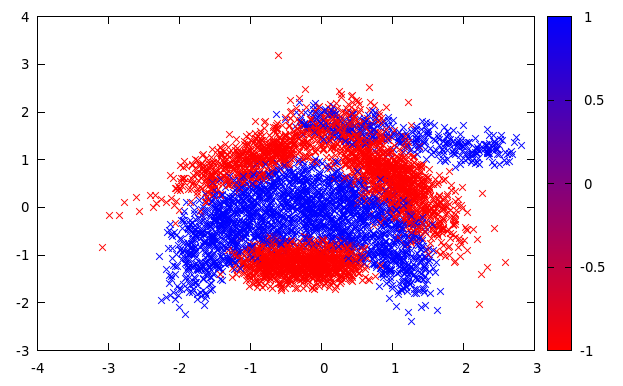
\includegraphics[scale=0.3]{banana.png}}
	\subfigure[CNN]{\label{fig:b}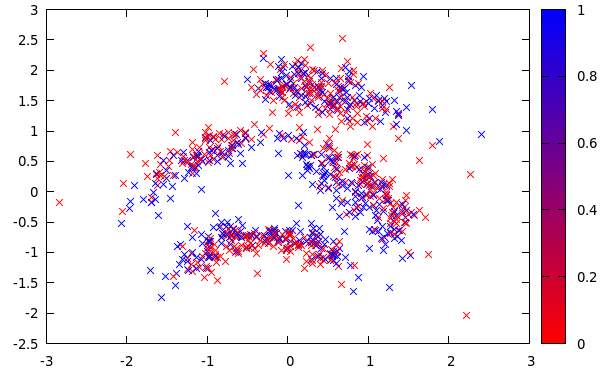
\includegraphics[scale=0.3]{CNN.png}}
	\subfigure[ENN]{\label{fig:c}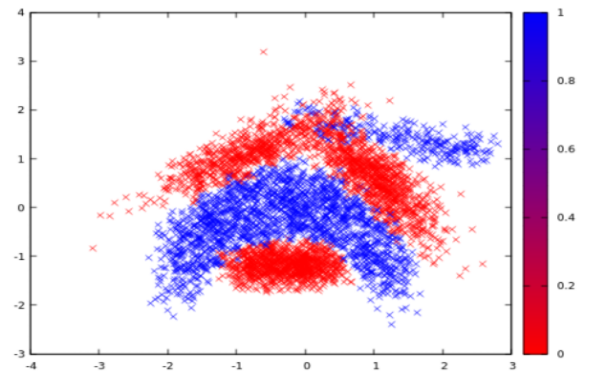
\includegraphics[scale=0.3]{ENN.png}}
	\subfigure[RSS]{\label{fig:d}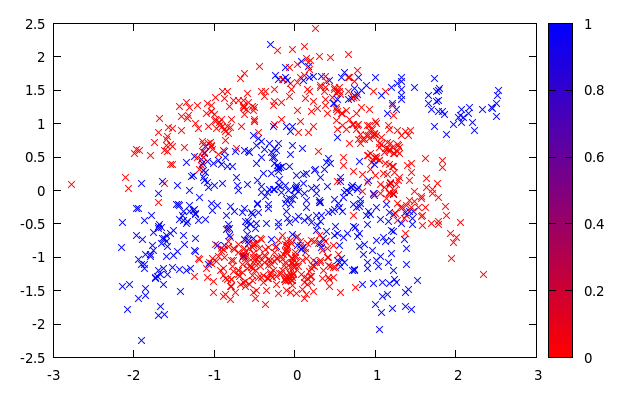
\includegraphics[scale=0.3]{RSS.png}}

\caption{Selección de puntos de las heurísticas}
\label{heu}
\end{figure}

Los experimentos fueron hechos con un procesador Intel(R) Core(TM) i5-3470 CPU @ 3.20GHz, 4 procesadores y 4GB de memoria RAM. Se utilizó C++ como lenguaje de programación y se compiló con GCC v.7.3.0.

\subsection{Resultados}

\subsubsection{Heurísticas}

El primer tipo de tablas que se presentan contienen los promedios en \emph{accuracy}, \emph{kappa}, reducción y tiempo de cómputo medido en segundos para cada heurística. \emph{Accuracy y kappa} se miden sobre los conjuntos de entrenamiento y prueba, la reducción mide el porcentaje de instancias eliminadas del conjunto original; a mayor \emph{accuracy, kappa} y reducción mejor es la metaheurística. Las pruebas fueron realizadas para los conjuntos pequeños, medianos y grandes por separado.

\begin{table}[h!]
\centering
\begin{tabular}{l c c c c c c}
\hline
\multirow{2}{*}{\textsc{Algoritmo}}
	& \multicolumn{2}{c}{\textsc{Accuracy}}
	& \multicolumn{2}{c}{\textsc{Kappa}}
	& \textsc{Reducción}
	& \textsc{Tiempo (seg)} \\
	& Training & Test
	& Training & Test \\ 
\hline
\hline

Pequeños\\
CNN & 0.9093 & 0.7447 & 0.8396 & 0.5404 & 0.7380 & 0.1351 \\
ENN & 0.8563 & 0.7924 & 0.7319 & 0.6120 & 0.2591 & 0.1815 \\
RSS & 0.8363 & 0.7499 & 0.6997 & 0.5426 & 0.7308 & 0.1231 \\

\hline

Medianos\\
CNN & 0.8944 & 0.7823 & 0.7611 & 0.5613 & 0.7437 & 0.7108 \\
ENN & 0.8402 & 0.7999 & 0.6842 & 0.5863 & 0.2861 & 1.2668 \\
RSS & 0.8619 & 0.7922 & 0.6822 & 0.5524 & 0.6477 & 0.9201 \\

\hline

Grandes\\
CNN & 0.8818 & 0.8158 & 0.7396 & 0.5587 & 0.8183 & 3.2853 \\
ENN & 0.9355 & 0.8895 & 0.7938 & 0.6463 & 0.1495 & 6.1658 \\
RSS & 0.9176 & 0.8731 & 0.7411 & 0.6007 & 0.7236 & 10.7264 \\


\hline
\end{tabular}
\caption{Promedios de heurísticas}
\label{heu}
\end{table}



Como se puede observar en la tabla \ref{heu}, ENN es la heurística que presenta el mayor \emph{accuracy y kappa}, esto se debe a que ENN es la heurística que menos reduce y por lo tanto el conjunto $S$ resultante se parece bastante al conjunto original, manteniendo su capacidad de representación casi intacta. Por otro lado CNN es la heurística que más reduce de las 3 con niveles muy parecidos en \emph{accuracy y kappa} a RSS en los conjuntos pequeños y medianos, pero con una diferencia en \emph{kappa} para los conjuntos grandes, en donde RSS supera por un 5\% a CNN; RSS por su parte presenta una tasa de reducción superior a ENN pero inferior a CNN. 

El conjunto $S$ proporcionado por CNN le da a la metaheurística utilizada una población bastante reducida con la cual trabajar, enfocada principalmente en los puntos bordes. ENN, en cambio, inicializa la población de la metaheurística con una gran cantidad de elementos, lo cual le deja a la metaheurística el trabajo de reducción. RSS le aporta a la metaheurística una población variada entre puntos internos y puntos bordes para trabajar.

\subsubsection{Metaheurísticas}


La tabla \ref{meta} presenta los promedios para las metaheurísticas con inicialización aleatoria. Además en las tablas \ref{wilcox-meta-peq} y \ref{wilcox-meta-med} se muestran los resultados de las pruebas de \emph{Wilcoxon} de rango con signo con un nivel de significacia de 1\%, donde se compara cada metaheurística en relación al \emph{accuracy, kappa}, reducción, \emph{0.5 * accuracy} + 0.5 * reducción y \emph{0.5 * kappa} + 0.5 * reducción. Donde la hipótesis nula implica que las medidas son estadísticamente iguales y la hipótesis alternativa indica que existe una diferencia real entre las medidas. 

\begin{table}[h!]
\centering
\begin{tabular}{l c c c c c c}
\hline
\multirow{2}{*}{\textsc{Algoritmo}}
	& \multicolumn{2}{c}{\textsc{Accuracy}}
	& \multicolumn{2}{c}{\textsc{Kappa}}
	& \textsc{Reducción}
	& \textsc{Tiempo (seg)} \\
	& Training & Test
	& Training & Test \\ 
\hline
\hline

Pequeños\\
GGA  & 0.8312 & 0.7525 & 0.7017 & 0.5557 & 0.5532 & 12.8250 \\
SSGA & 0.8654 & 0.7716 & 0.7635 & 0.5917 & 0.8432 & 0.6655 \\
MA   & 0.8570 & 0.7918 & 0.7440 & 0.6216 & 0.9561 & 4.1047 \\
CHC & 0.8446 & 0.7843 & 0.7172 & 0.6084 & 0.9466 & 0.5266 \\

\hline

Medianos\\
GGA  & 0.8702 & 0.7982 & 0.7375 & 0.5812 & 0.5641 & 110.0812 \\
SSGA & 0.8431 & 0.8029 & 0.6676 & 0.5871 & 0.8392 & 3.5589 \\
MA   & 0.8057 & 0.7908 & 0.5825 & 0.5564 & 0.9624 & 73.3461 \\
CHC  & 0.8313 & 0.8115 & 0.6347 & 0.5986 & 0.9455 & 2.8843 \\

\hline
Grandes\\
GGA  & 0.9316 & 0.8644 & 0.7994 & 0.6014 & 0.5050 & 672.0273 \\
SSGA & 0.8911 & 0.8743 & 0.6953 & 0.6201 & 0.8056 & 27.6637 \\
MA   & 0.8904 & 0.8999 & 0.6499 & 0.6510 & 0.9973 & 256.1432 \\
CHC  & 0.8961 & 0.8934 & 0.6614 & 0.6506 & 0.9615 & 16.8665 \\

\hline
\end{tabular}
\caption{Promedios de las metaheurísticas}
\label{meta}
\end{table}


\begin{figure}[h!]

	\centering
	\subfigure[\emph{Accuracy} + reducción]{\label{fig:a}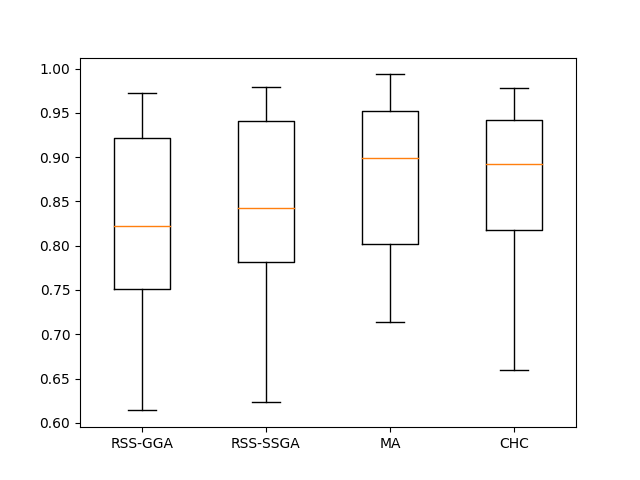
\includegraphics[scale=0.4]{acc_small.png}}
	\subfigure[\emph{kappa} + reducción]{\label{fig:b}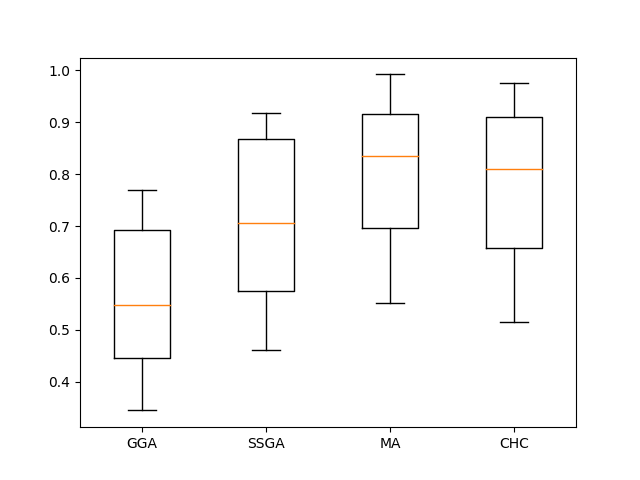
\includegraphics[scale=0.4]{kappa_small.png}}

\caption{Boxplots de las metaheurísticas para los conjuntos pequeños}
\label{small-heuristics}
\end{figure}

\begin{figure}[h!]

	\centering
	\subfigure[\emph{Accuracy} + reducción]{\label{fig:a}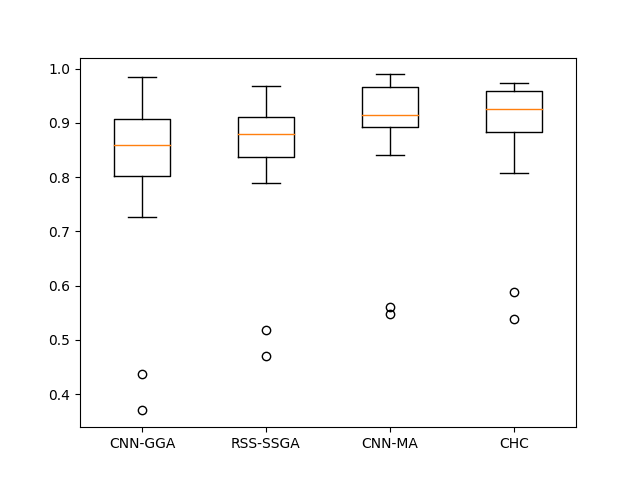
\includegraphics[scale=0.4]{acc_medium.png}}
	\subfigure[\emph{kappa} + reducción]{\label{fig:b}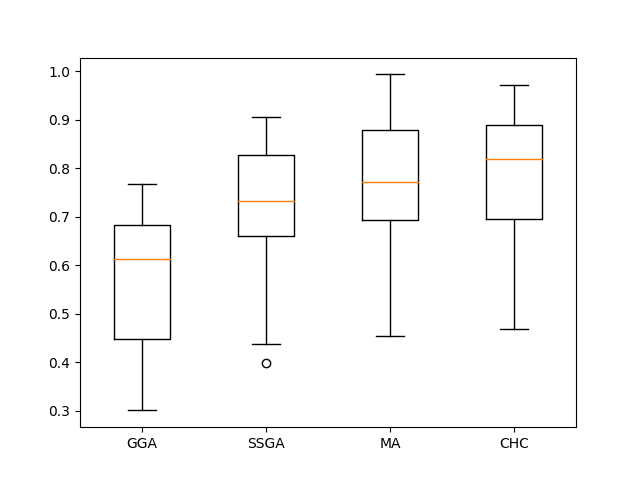
\includegraphics[scale=0.4]{kappa_medium.png}}

\caption{Boxplots de las metaheurísticas para los conjuntos medianos}
\label{medium-heuristics}
\end{figure}


\begin{table}[h!]
\centering
\begin{adjustbox}{max width =\textwidth}
\begin{tabular}{l c c c c c}
\hline
	\textsc{Algoritmo}
	& \multicolumn{1}{c}{\textsc{Accuracy}}
	& \multicolumn{1}{c}{\textsc{Kappa}}
	& \multicolumn{1}{c}{\textsc{Reducción}} 
	& \multicolumn{1}{c}{\textsc{Accuracy + reducción}} 
	& \multicolumn{1}{c}{\textsc{kappa + reducción}} \\
\hline
\hline

 & p-valor & p-valor & p-valor & p-valor & p-valor \\

GGA \\
vsSSGA & 1.855e-02 & 2.142e-02 & 1.228e-05 & 1.229e-05 & 1.229e-05 \\
vsMA & 7.421e-03 & 2.643e-02 & 1.229e-05 & 1.229e-05 & 1.229e-05 \\
vsCHC & 3.822e-03 & 3.822e-03 & 1.228e-05 & 1.229e-05 & 1.229e-05 \\

\hline

SSGA \\
vsMA & 1.373e-01 & 1.615e-01 & 1.229e-05 & 1.229e-05 & 2.543e-05 \\
vsCHC & 1.779e-01 & 3.395e-01 & 1.228e-05 & 1.229e-05 & 2.001e-05 \\

\hline

MA \\
vsCHC & 1.873e-01 & 1.425e-01 & 8.401e-01 & 6.934e-02 & 7.800e-02 \\ 

\hline

\end{tabular}
\end{adjustbox}
\caption[Pruebas de \emph{Wilcoxon} entre las metaheurísticas para conjuntos pequeños]{$p$-valor de pruebas de rangos con signo de \emph{Wilcoxon} para las distintas metaheurísticas sobre conjuntos pequeños}
\label{wilcox-meta-peq}
\end{table}

\begin{table}[h!]
\centering
\begin{adjustbox}{max width =\textwidth}
\begin{tabular}{l c c c c c}
\hline
	\textsc{Algoritmo}
	& \multicolumn{1}{c}{\textsc{Accuracy}}
	& \multicolumn{1}{c}{\textsc{Kappa}}
	& \multicolumn{1}{c}{\textsc{Reducción}} 
	& \multicolumn{1}{c}{\textsc{Accuracy + reducción}} 
	& \multicolumn{1}{c}{\textsc{kappa + reducción}} \\
\hline
\hline

 & p-valor & p-valor & p-valor & p-valor & p-valor \\

GGA \\
vsSSGA & 9.359e-01 & 4.688e-01 & 1.318e-04 & 1.318e-04 & 1.318e-04 \\
vsMA & 8.405e-01 & 3.547e-01 & 1.318e-04 & 1.318e-04 & 1.318e-04 \\
vsCHC & 5.197e-01 & 7.172e-01 & 1.318e-04 & 1.318e-04 & 1.318e-04 \\

\hline

SSGA \\
vsMA & 1.842e-01 & 1.365e-01 & 1.318e-04 & 1.318e-04 & 1.318e-04 \\
vsCHC & 2.122e-01 & 4.939e-01 & 1.316e-04 & 1.318e-04 & 1.316e-04 \\

\hline

MA \\
vsCHC & 1.57e-02 & 5.338e-02 & 9.100e-02 & 6.009e-01 & 7.172e-01 \\ 

\hline


\end{tabular}
\end{adjustbox}
\caption[Pruebas de \emph{Wilcoxon} entre las metaheurísticas para conjuntos pequeños]{$p$-valor de pruebas de rangos con signo de \emph{Wilcoxon} para las distintas metaheurísticas sobre conjuntos medianos}
\label{wilcox-meta-med}
\end{table}


Las figuras \ref{small-heuristics} y \ref{medium-heuristics} muestran que MA y CHC tienen la mejor relación entre \emph{accuracy, kappa} y reducción tanto para los conjuntos pequeños como medianos. Cuando se revisa la tabla con los promedios y los p-valores \ref{meta} \ref{wilcox-meta-peq}, para los conjuntos pequeños se tiene que las 4 metaheurísticas presentan niveles similares de \emph{accuracy y kappa}, destacando MA y CHC por tener los valores más elevados. La diferencia se encuentra en la reducción, donde MA y CHC superan a SSGA y GGA.

Para los conjuntos medianos, las tablas \ref{meta} y \ref{wilcox-meta-med} muestran un comportamiento similar que los conjuntos pequeños; con la diferencia de que el \emph{accuracy y kappa} son estadísticamente similares entre todas las metaheurísticas y la mayor reducción la presentan CHC y MA. Para los conjuntos grandes, la tabla \ref{meta} muestra que CHC y MA presentan \emph{accuracy, kappa} y reducción superiores a SSGA y GGA. Con estos resultados se puede deducir que el principal factor que influye entre las relaciones \emph{accuracy} + reducción y \emph{kappa} + reducción es la reducción, que es la medida que presenta las diferencias más marcadas entre las metaheurísticas.


\subsubsection{Variaciones de las metaheurísticas}

A continuación se pasa a combinar las heurísticas con las metaheurísticas. La idea es evaluar las variaciones de cada metaheurística por separado, de tal manera de que se se identifique cuál heurística beneficia más a la metaheurística. La notación en la columna de ``\textsc{Algoritmo}'' indica primero qué heurística se usó para inicializar la población y le sigue la metaheurística usada; un ejemplo es CNN-GGA, que indica que CNN es la heurística usada para inicializar la población de la metaheurística GGA. Para el caso de usar una población incial aleatoria, se coloca simplemente el nombre de la metaheurística.


\paragraph{Conjuntos pequeños}

\begin{figure}[h!]

	\centering
	\subfigure[\emph{Accuracy} + reducción]{\label{fig:a}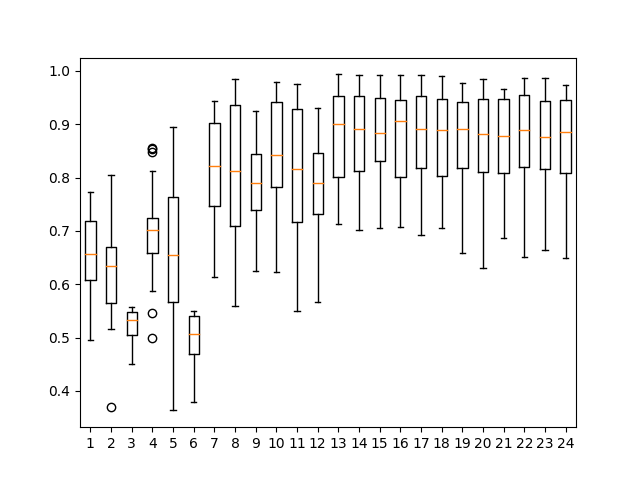
\includegraphics[scale=0.4]{acc_small_all.png}}
	\subfigure[\emph{kappa} + reducción]{\label{fig:b}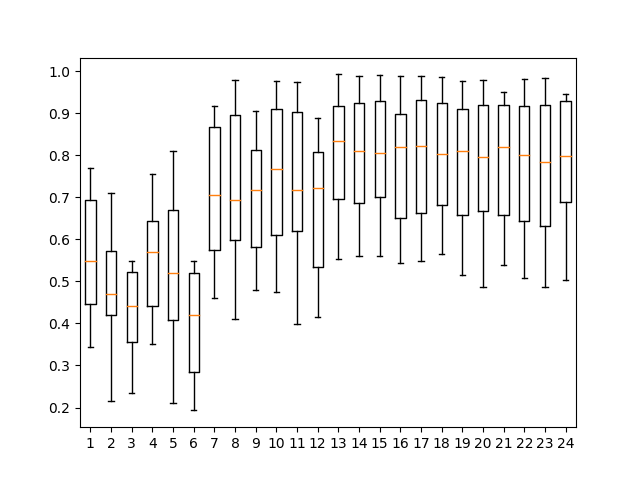
\includegraphics[scale=0.4]{kappa_small_all.png}}

\caption{Boxplots de las variaciones de las metaheurísticas para los conjuntos pequeños}
\label{small-all}
\end{figure}

\begin{table}[h!]
\centering
\begin{tabular}{l c c c c c c}
\hline
\multirow{2}{*}{\textsc{Algoritmo}}
	& \multicolumn{2}{c}{\textsc{Accuracy}}
	& \multicolumn{2}{c}{\textsc{Kappa}}
	& \textsc{Reducción}
	& \textsc{Tiempo (seg)} \\
	& Training & Test
	& Training & Test \\ 
\hline
\hline

GGA         & 0.8312 & 0.7525 & 0.7017 & 0.5557 & 0.5532 & 12.8250 \\
CNN-GGA     & 0.5736 & 0.4911 & 0.3525 & 0.2151 & 0.7491 & 33.4671 \\
ENN-GGA     & 0.8533 & 0.7891 & 0.7327 & 0.6093 & 0.2611 & 14.6024 \\
\textbf{RSS-GGA}     & \textbf{0.6626} & \textbf{0.6177} & \textbf{0.4044} & \textbf{0.3263} & \textbf{0.7717} & \textbf{21.5376} \\
CNN-RSS-GGA & 0.7883 & 0.6809 & 0.6353 & 0.4472 & 0.6221 & 43.1002 \\
ENN-RSS-GGA & 0.8973 & 0.7872 & 0.8182 & 0.6063 & 0.1994 & 36.5439 \\

\hline

SSGA & 0.8654 & 0.7716 & 0.7635 & 0.5917 & 0.8432 & 0.6655 \\
CNN-SSGA & 0.8791 & 0.7695 & 0.7840 & 0.5815 & 0.8425 & 1.2187 \\
ENN-SSGA & 0.8733 & 0.7919 & 0.7683 & 0.6112 & 0.7823 & 0.8601 \\
\textbf{RSS-SSGA} & \textbf{0.8581} & \textbf{0.7726} & \textbf{0.7460} & \textbf{0.5905} & \textbf{0.8958} &\textbf{1.0116} \\
CNN-RSS-SSGA & 0.8808 & 0.7742 & 0.7884 & 0.5974 & 0.8373 & 1.9109 \\
EEN-RSS-SSGA & 0.8843 & 0.7890 & 0.7904 & 0.6134 & 0.7586 & 1.6563 \\

\hline

\textbf{MA}   & \textbf{0.8570} & \textbf{0.7918} & \textbf{0.7440} & \textbf{0.6216} & \textbf{0.9561} & \textbf{4.1047} \\
CNN-MA & 0.8653 & 0.7987 & 0.7519 & 0.6307 & 0.9486 & 5.9638 \\
ENN-MA & 0.8666 & 0.7930 & 0.7576 & 0.6215 & 0.9534 & 4.2491 \\
RSS-MA & 0.8446 & 0.7795 & 0.7137 & 0.5903 & 0.9630 & 4.6391 \\
CNN-RSS-MA  & 0.8639 & 0.7848 & 0.7538 & 0.6090 & 0.9507 & 8.9884 \\
ENN-RSS-MA & 0.8736 & 0.7942 & 0.7716 & 0.6268 & 0.9474 & 8.3942 \\

\hline

\textbf{CHC} & \textbf{0.8446} & \textbf{0.7843} & \textbf{0.7172} & \textbf{0.6084} & \textbf{0.9466} & \textbf{0.5266} \\
CNN-CHC & 0.8495 & 0.7812 & 0.7269 & 0.6027 & 0.9385 & 0.7891 \\
ENN-CHC & 0.8429 & 0.7863 & 0.7179 & 0.6132 & 0.9424 & 0.7445 \\
RSS-CHC & 0.8383 & 0.7779 & 0.6963 & 0.5836 & 0.9546 & 0.7137 \\
CNN-RSS-CHC  & 0.8442 & 0.7794 & 0.7099 & 0.5864 & 0.9437 & 1.1144 \\
ENN-RSS-CHC & 0.8484 & 0.7846 & 0.7224 & 0.6030 & 0.9333 & 1.0723 \\

\hline
\end{tabular}
\caption{Promedios de las distintas variaciones de cada metaheurística para los conjuntos pequeños}
\label{peq-all}
\end{table}


\begin{table}[h!]
\centering
\begin{adjustbox}{max width =\textwidth}
\begin{tabular}{l c c c c c}
\hline
	\textsc{Algoritmo}
	& \multicolumn{1}{c}{\textsc{Accuracy}}
	& \multicolumn{1}{c}{\textsc{Kappa}}
	& \multicolumn{1}{c}{\textsc{Reducción}} 
	& \multicolumn{1}{c}{\textsc{Accuracy + reducción}} 
	& \multicolumn{1}{c}{\textsc{kappa + reducción}} \\
\hline
\hline

 & p-valor & p-valor & p-valor & p-valor & p-valor \\

RSS-GGA\\
vsGGA & 7.224e-05 & 6.451e-05 & 1.773e-05 & 6.446e-05 & 9.036e-01 \\ 
vsCNN-RSS-GGA & 8.481e-04 & 1.405e-04 & 2.257e-05 & 3.216e-03 & 4.758e-01 \\ 

\hline 

GGA\\
vsCNN-RSS-GGA & 4.927e-03 & 7.423e-03 & 9.263e-02 & 8.086e-01 & 3.130e-01 \\ 

\hline

\end{tabular}
\end{adjustbox}
\caption[Pruebas de \emph{Wilcoxon} entre GGA y variaciones para conjuntos pequeños]{$p$-valor de pruebas de rangos con signo de \emph{Wilcoxon} para GGA sobre conjuntos pequeños}
\label{wilcox-gga-peq}
\end{table}

\begin{table}[h!]
\centering
\begin{adjustbox}{max width =\textwidth}
\begin{tabular}{l c c c c c}
\hline
	\textsc{Algoritmo}
	& \multicolumn{1}{c}{\textsc{Accuracy}}
	& \multicolumn{1}{c}{\textsc{Kappa}}
	& \multicolumn{1}{c}{\textsc{Reducción}} 
	& \multicolumn{1}{c}{\textsc{Accuracy + reducción}} 
	& \multicolumn{1}{c}{\textsc{kappa + reducción}} \\

\hline
\hline

 & p-valor & p-valor & p-valor & p-valor & p-valor \\

RSS-SSGA\\
vsSSGA & 6.865e-01 & 9.250e-01 & 1.772e-05 & 1.941e-04 & 4.162e-03 \\ 
vsCNN-SSGA & 5.774e-01 & 5.998e-01 & 2.692e-05 & 1.186e-03 & 1.430e-03 \\
vsCNN-RSS-SSGA & 6.476e-01 & 4.073e-01 & 1.229e-05 & 8.085e-05 & 2.699e-03 \\

\hline

SSGA\\
vsCNN-SSGA & 7.366e-01 & 5.449e-01 & 9.317e-01 & 9.893e-01 & 8.191e-01 \\  
vsCNN-RSS-SSGA & 7.570e-01 & 6.281e-01 & 6.964e-01 & 9.250e-01 & 7.366e-01 \\ 

\hline

CNN-SSGA\\
vsCNN-RSS-SSGA & 2.418e-01 & 4.797e-02 & 5.933e-02 & 9.464e-01 & 1.658e-01 \\

\hline 

\end{tabular}
\end{adjustbox}
\caption[Pruebas de \emph{Wilcoxon} entre SSGA y variaciones para conjuntos pequeños]{$p$-valor de pruebas de rangos con signo de \emph{Wilcoxon} para SSGA sobre conjuntos pequeños}
\label{wilcox-SSGA-peq}
\end{table}

\begin{table}[h!]
\centering
\begin{adjustbox}{max width =\textwidth}
\begin{tabular}{l c c c c c}
\hline
	\textsc{Algoritmo}
	& \multicolumn{1}{c}{\textsc{Accuracy}}
	& \multicolumn{1}{c}{\textsc{Kappa}}
	& \multicolumn{1}{c}{\textsc{Reducción}} 
	& \multicolumn{1}{c}{\textsc{Accuracy + reducción}} 
	& \multicolumn{1}{c}{\textsc{kappa + reducción}} \\

\hline
\hline

 & p-valor & p-valor & p-valor & p-valor & p-valor \\

MA\\
vsCNN-MA     & 6.682e-01 & 6.892e-01 & 1.430e-03 & 6.668e-01 & 9.678e-01 \\ 
vsENN-MA     & 9.678e-01 & 9.036e-01 & 1.617e-01 & 5.629e-01 & 9.036e-01 \\
vsRSS-MA     & 1.035e-01 & 1.094e-01 & 2.469e-03 & 4.432e-01 & 2.418e-01 \\ 
vsCNN-RSS-MA & 1.353e-01 & 6.934e-02 & 6.932e-02 & 4.215e-02 & 3.704e-02 \\ 
vsENN-RSS-MA & 6.034e-01 & 3.967e-01 & 3.404e-03 & 3.002e-01 & 6.766e-01 \\

\hline

CNN-MA\\
vsENN-MA & 1.918e-01 & 4.118e-01 & 1.261e-01 & 7.751e-01 & 9.893e-01 \\ 
vsRSS-MA & 2.227e-02 & 1.516e-02 & 4.073e-05 & 5.449e-01 & 1.155e-01 \\ 
vsCNN-RSS-MA & 8.571e-03 & 2.299e-02 & 2.879e-01 & 3.243e-02 & 2.831e-02 \\ 
vsENN-RSS-MA & 3.819e-01 & 5.629e-01 & 3.129e-01 & 3.194e-01 & 3.819e-01 \\ 

\hline

ENN-MA\\
vsRSS-MA & 2.209e-01 & 1.919e-01 & 2.956e-04 & 9.036e-01 & 5.449e-01 \\ 
vsCNN-RSS-MA & 1.742e-01 & 3.129e-01 & 6.265e-01 & 1.855e-02 & 1.155e-01 \\ 
vsENN-RSS-MA & 9.464e-01 & 6.964e-01 & 1.479e-03 & 2.641e-01 & 8.401e-01 \\ 

\hline

RSS-MA\\
vsCNN-RSS-MA & 4.576e-01 & 2.478e-01 & 1.822e-05 & 3.458e-01 & 8.415e-01 \\
vsENN-RSS-MA & 6.746e-02 & 3.955e-02 & 3.220e-05 & 7.982e-01 & 3.674e-01 \\ 

\hline

CNN-RSS-MA\\
vsENN-RSS-MA & 3.002e-01 & 1.829e-01 & 1.793e-01 & 9.250e-01 & 3.674e-01 \\ 

\hline 

\end{tabular}
\end{adjustbox}
\caption[Pruebas de \emph{Wilcoxon} entre MA y variaciones para conjuntos pequeños]{$p$-valor de pruebas de rangos con signo de \emph{Wilcoxon} para MA sobre conjuntos pequeños}
\label{wilcox-MA-peq}
\end{table}


\begin{table}[h!]
\centering
\begin{adjustbox}{max width =\textwidth}
\begin{tabular}{l c c c c c}
\hline
	\textsc{Algoritmo}
	& \multicolumn{1}{c}{\textsc{Accuracy}}
	& \multicolumn{1}{c}{\textsc{Kappa}}
	& \multicolumn{1}{c}{\textsc{Reducción}} 
	& \multicolumn{1}{c}{\textsc{Accuracy + reducción}} 
	& \multicolumn{1}{c}{\textsc{kappa + reducción}} \\
\hline
\hline

 & p-valor & p-valor & p-valor & p-valor & p-valor \\

CHC\\
vsCNN-CHC     & 3.967e-01 & 4.432e-01 & 1.188e-02 & 1.658e-01 & 1.742e-01 \\ 
vsENN-CHC     & 8.823e-01 & 8.506e-01 & 4.245e-02 & 3.674e-01 & 4.593e-01 \\ 
vsRSS-CHC     & 5.629e-01 & 3.533e-01 & 6.642e-03 & 7.982e-01 & 6.571e-01 \\ 
vsCNN-RSS-CHC & 3.674e-01 & 1.284e-01 & 2.699e-01 & 4.593e-01 & 2.528e-01 \\ 
vsENN-RSS-CHC & 8.639e-01 & 9.464e-01 & 6.739e-04 & 9.797e-02 & 2.109e-01 \\ 

\hline

CNN-CHC\\
vsENN-CHC & 2.418e-01 & 3.395e-01 & 8.823e-01 & 6.571e-01 & 5.812e-01 \\
vsRSS-CHC & 9.515e-01 & 4.118e-01 & 9.067e-05 & 1.658e-01 & 9.893e-01 \\
vsCNN-RSS-CHC & 9.886e-01 & 3.606e-01 & 2.418e-01 & 7.164e-01 & 8.191e-01 \\ 
vsENN-RSS-CHC & 3.615e-01 & 5.633e-01 & 2.528e-01 & 9.036e-01 & 7.982e-01 \\ 

\hline

ENN-CHC\\
vsRSS-CHC & 4.432e-01 & 3.260e-01 & 1.498e-03 & 4.273e-01 & 9.464e-01 \\ 
vsCNN-RSS-CHC & 5.098e-01 & 3.002e-01 & 6.766e-01 & 9.893e-01 & 5.449e-01 \\ 
vsENN-RSS-CHC & 6.682e-01 & 3.819e-01 & 2.380e-02 & 2.109e-01 & 1.285e-01 \\ 

\hline

RSS-CHC\\
vsCNN-RSS-CHC & 7.672e-01 & 6.186e-01 & 1.756e-03 & 6.092e-01 & 9.464e-01 \\ 
vsENN-RSS-CHC & 4.405e-01 & 3.819e-01 & 1.127e-04 & 2.418e-01 & 7.366e-01 \\ 

\hline

CNN-RSS-CHC\\
vsENN-RSS-CHC & 7.317e-01 & 6.071e-01 & 1.913e-02 & 6.186e-01 & 6.766e-01 \\ 

\hline 

\end{tabular}
\end{adjustbox}
\caption[Pruebas de \emph{Wilcoxon} entre CHC y variaciones para conjuntos pequeños]{$p$-valor de pruebas de rangos con signo de \emph{Wilcoxon} para CHC sobre conjuntos pequeños}
\label{wilcox-CHC-peq}
\end{table}

La figura \ref{small-all} muestra \emph{boxplots} de todas las variaciones de metaheurísticas para los conjuntos pequeños, de izquierda a derecha los \emph{boxplots} representan las siguientes variaciones: '1':GGA, '2':CNN-GGA, '3':ENN-GGA, '4':RSS-GGA, '5':CNN-RSS-GGA, '6':ENN-RSS-GGA, '7':SSGA, '8':CNN-SSGA, '9':ENN-SSGA, '10':RSS-SSGA, '11':CNN-RSS-SSGA, '12':ENN-RSS-SSGA, '13':MA, '14':CNN-MA, '15':ENN-MA, '16':RSS-MA, '17':CNN-RSS-MA, '18':ENN-RSS-MA, '19':CHC, '20':CNN-CHC, '21':ENN-CHC, '22':RSS-CHC, '23':CNN-RSS-CHC y '24':ENN-RSS-CHC.

Los \emph{boxplots} que van del 1 al 6 de la figura \ref{small-all} muestran que GGA, RSS-GGA y CNN-RSS-GGA presentan valores muy similares en \emph{accuracy} + reducción. Cuando se evalúan los p-valores la tabla \ref{wilcox-gga-peq} se nota que GGA y CNN-RSS-GGA son estadísticamente similares, mientras que RSS-GGA es distinto de los otros dos métodos. Cuando se revisan los promedios en la tabla \ref{peq-all} se nota que hay diferencias marcadas en \emph{accuracy} y reducción; donde RSS-GGA mantiene buenos niveles de \emph{accuracy} y posee la mayor tasa de reducción. 

Con respecto a \emph{kappa} + reducción para los conjuntos pequeños, GGA, RSS-GGA y CNN-RSS-GGA presentan niveles muy similares en la figura \ref{small-all}, lo cual es respaldado por los p-valores de la tabla \ref{wilcox-gga-peq}, que muestran que los tres métodos son estadísticamente similares.

Al evaluar el tiempo de cómputo entre las distintas variantes de GGA, se tiene que ENN-GGA y RSS-GGA son las versiones más rápidas, tardando 1.7774 y 8.7126 segundos más en devolver un resultado que la inicialización aleatoria. 

De los resultados anteriores RSS-GGA resalta como la mejor opción entre las variaciones de GGA para los conjuntos pequeños; RSS-GGA presenta 21.85\% más reducción que la inicialización aleatoria a cambio de 8.7126 segundos más de tiempo de cómputo.

Los \emph{boxplots} que van del 7 al 12 de la figura \ref{small-all} muestran valores muy similares en \emph{accuracy} + reducción y \emph{kappa} + reducción entre SSGA, CNN-SSGA, RSS-SSGA y CNN-RSS-SSGA; los p-valores en la tabla \ref{wilcox-SSGA-peq} corroboran que SSGA, CNN-SSGA y CNN-RSS-SSGA presentan medias estadísticamente iguales, mientras que RSS-SSGA presenta valores distintos para las dos medidas. La tabla \ref{peq-all} muestra que las cuatro variaciones muestran valores muy similares para \emph{accuracy y kappa}, pero RSS-SSGA posee una mayor tasa de reducción con 89.58\%.   

Con respecto a los tiempos de cómputo de las variantes de SSGA se tiene que ENN-SSGA y RSS-SSGA son las versiones más rápidas, tardando 0.2 y 0.35 segundos más que la inicialización aleatoria en devolver un resultado.

De los resultados anteriores, RSS-SSGA se puede identificar como la mejor variación de SSGA para los conjuntos pequeños, donde se presenta un \emph{accuracy y kappa} prácticamente iguales a SSGA, con una diferencia en reducción de 5.26\% a favor de RSS-SSGA.

Los \emph{boxplots} que van desde el 13 al 18 de la figura \ref{small-all} muestran valores muy similares entre todas las variaciones de MA para \emph{accuracy} + reducción y para \emph{kappa} + reducción. Ninguna variante destaca sobre otra, los p-valores de la tabla \ref{wilcox-MA-peq} confirman que todas las variaciones son estadísticamente similares y en la tabla \ref{peq-all}, no se nota una diferencia real entre los promedios.

En este sentido para elegir cual es la mejor variante de entre todas se decide en función al tiempo de cómputo que les toma para devolver una respuesta. Es por eso que para los conjuntos pequeños, una inicialización aleatoria es la mejor opción al presentar los menores tiempos.

Los \emph{boxplots} que van desde el 19 al 24 de la figura \ref{small-all} muestran un comportamiento similar para todas las variantes de CHC como el visto para MA, en donde todas presentan valores similares en \emph{accuracy} + reducción y \emph{kappa} + reducción. Los p-valores de la tabla \ref{wilcox-CHC-peq} muestran que todas las variantes tienen valores estadísticamente similares. La tabla \ref{peq-all} corrobora la noción de que para los conjuntos pequeños, los resultados en \emph{accuracy, kappa} y reducción son similares para todas las variantes.

Ya que todas las variantes  presentan valores similares entre \emph{accuracy, kappa} y reducción, se elige cuál es la mejor en función al tiempo de cómputo, en cuyo caso CHC con inicialización aleatoria presenta el menor tiempo en todas las instancias y por lo tanto es la variante preferida para los conjuntos pequeños.

\begin{table}[h!]
\centering
\begin{adjustbox}{max width =\textwidth}
\begin{tabular}{l c c c c c}
\hline
	\textsc{Algoritmo}
	& \multicolumn{1}{c}{\textsc{Accuracy}}
	& \multicolumn{1}{c}{\textsc{Kappa}}
	& \multicolumn{1}{c}{\textsc{Reducción}} 
	& \multicolumn{1}{c}{\textsc{Accuracy + reducción}} 
	& \multicolumn{1}{c}{\textsc{kappa + reducción}} \\
\hline
\hline

RSS-GGA\\
vsRSS-SSGA & 4.574e-05 & 6.451e-05 & 4.574e-05 & 1.229e-05 & 1.229e-05 \\
vsMA       & 2.001e-05 & 3.624e-05 & 1.390e-05 & 1.229e-05 & 1.229e-05 \\
vs CHC     & 2.257e-05 & 2.001e-05 & 2.541e-05 & 1.229e-05 & 1.229e-05 \\

\hline 

RSS-SSGA\\
vsMA  & 3.243e-02 & 5.437e-02 & 1.822e-05 & 1.405e-04 & 6.022e-04 \\
vsCHC & 8.648e-02 & 1.353e-01 & 1.571e-05 & 1.941e-04 & 1.720e-03 \\

\hline

MA\\
vsCHC & 1.873e-01 & 1.425e-01 & 8.401e-01 & 6.934e-02 & 7.800e-02 \\

\hline

\end{tabular}
\end{adjustbox}
\caption[Pruebas de \emph{Wilcoxon} entre las mejores variaciones de cada metaheurística para conjuntos pequeños]{$p$-valor de pruebas de rangos con signo de \emph{Wilcoxon} para las mejores variantes de las metaheurísticas sobre conjuntos pequeños}
\label{wilcox-best-peq}
\end{table}

\begin{table}[h!]
\centering
\begin{adjustbox}{max width =\textwidth}
\begin{tabular}{l c c|l c c|l c c}
\hline
\multicolumn{3}{c|}{\textsc{Accuracy + Reducción}}
	& \multicolumn{3}{c|}{\textsc{Kappa + Reducción}}
	& \multicolumn{3}{c}{\textsc{Tiempo}} \\
\hline
Algoritmo & Rank & Mejor & Algoritmo & Rank & Mejor & Algoritmo & Rank & Mejor \\
\hline
\hline

MA           & 5.38  & 5 & CNN-MA       & 5.26  & 4  & CHC          & 1.34 & 20 \\
ENN-MA       & 5.46  & 2 & ENN-MA       & 5.53  & 0  & SSGA         & 2.57 & 4 \\
CNN-MA       & 5.57  & 4 & MA           & 5.57  & 5  & RSS-CHC      & 3.26 & 0 \\
RSS-MA       & 6.07  & 6 & ENN-RSS-MA   & 6.00  & 3  & ENN-CHC      & 4.53 & 0 \\
ENN-RSS-MA   & 6.30  & 3 & RSS-MA       & 6.76  & 6  & CNN-CHC      & 4.96 & 0 \\
RSS-CHC      & 6.80  & 1 & CNN-RSS-MA   & 7.07  & 0  & ENN-SSGA     & 5.57 & 1 \\
CNN-RSS-MA   & 6.96  & 0 & ENN-CHC      & 7.46  & 2  & RSS-SSGA     & 7.23 & 1 \\
CHC          & 7.07  & 0 & CHC          & 7.50  & 1  & CNN-SSGA     & 7.73 & 0 \\
ENN-CHC      & 7.53  & 0 & RSS-CHC      & 7.96  & 1  & ENN-RSS-CHC  & 8.88 & 0 \\
CNN-RSS-CHC  & 7.65  & 2 & CNN-RSS-CHC  & 8.07  & 2  & CNN-RSS-CHC  & 9.26 & 0 \\
ENN-RSS-CHC  & 7.88  & 2 & ENN-RSS-CHC  & 8.26  & 1  & ENN-RSS-SSGA & 11.80 & 0 \\
CNN-CHC      & 8.73  & 1 & CNN-CHC      & 8.84  & 1  & CNN-RSS-SSGA & 12.38 & 0 \\
RSS-SSGA     & 12.07 & 0 & RSS-SSGA     & 11.92 & 0  & MA           & 13.53 & 0 \\
CNN-SSGA     & 14.53 & 0 & SSGA         & 14.30 & 0  & ENN-MA       & 13.69 & 0 \\
SSGA         & 14.88 & 0 & CNN-RSS-SSGA & 14.26 & 0  & RSS-MA       & 14.15 & 0 \\
CNN-RSS-SSGA & 15.07 & 0 & CNN-SSGA     & 14.46 & 0  & CNN-MA       & 15.30 & 0 \\
ENN-SSGA     & 16.11 & 0 & ENN-SSGA     & 15.26 & 0  & CNN-RSS-MA   & 17.65 & 0 \\
ENN-RSS-SSGA & 17.26 & 0 & ENN-RSS-SSGA & 16.42 & 0  & ENN-RSS-MA   & 17.80 & 0 \\
RSS-GGA      & 19.11 & 0 & GGA          & 20.15 & 0  & GGA          & 19.84 & 0 \\
GGA          & 20.73 & 0 & RSS-GGA      & 20.19 & 0  & ENN-GGA      & 20.38 & 0 \\
CNN-RSS-GGA  & 20.84 & 0 & CNN-RSS-GGA  & 20.88 & 0  & CNN-GGA      & 20.42 & 0 \\
CNN-GGA      & 21.30 & 0 & CNN-GGA      & 21.69 & 0  & ENN-RSS-GGA  & 23.26 & 0 \\
ENN-GGA      & 22.73 & 0 & ENN-GGA      & 22.53 & 0  & RSS-GGA      & 21.00 & 0 \\
ENN-RSS-GGA  & 23.84 & 0 & ENN-RSS-GGA  & 23.53 & 0  & CNN-RSS-GGA  & 23.34 & 0 \\



\hline
\end{tabular}
\end{adjustbox}
\caption{Rangos de las metaheurísticas en \emph{accuracy + reducción}, \emph{kappa + reducción} y tiempo para los conjuntos pequeños}
\label{rank-peq}
\end{table} 


Teniendo las mejores variaciones de cada metaheurística para los conjuntos pequeños: RSS-GGA, RSS-SSGA, MA y CHC, se hace una comparación entre ellos para determinar cuál es la mejor opción. La figura \ref{small-all} muestra que '13':MA y '19':CHC presentan los mejores valores en \emph{accuracy} + reducción y \emph{kappa} + reducción. La tabla \ref{wilcox-best-peq} muestra que MA y CHC son estadísticamente similares y esto se puede apreciar al comparar los valores de la tabla \ref{peq-all}. 

La tabla \ref{rank-peq} ordena todas las metaheurísticas y sus variaciones por el rango asignado de mayor a menor sus resultados por instancia. La columna de  \emph{``rank''} muestra el rango promedio en el que quedó cada metaheurística, la columna de \emph{``best''} indica en cuántos conjuntos dicha metaheurística quedó como la mejor opción.

En la tabla \ref{rank-peq} las variaciones de MA y CHC comparten los primeros puestos al tener los mejores valores en \emph{accuracy, kappa} y reducción. La diferencia principal entre ambas radica en el tiempo de cómputo, donde las variaciones de MA son más lentas que las de CHC y SSGA, mientras que las variaciones de CHC son las más rápidas entre todas. Lo cual hace a CHC con inicialización aleatoria la opción a elegir para los conjuntos pequeños.

\paragraph{Conjuntos medianos}

\begin{figure}[h!]

	\centering
	\subfigure[\emph{Accuracy} + reducción]{\label{fig:a}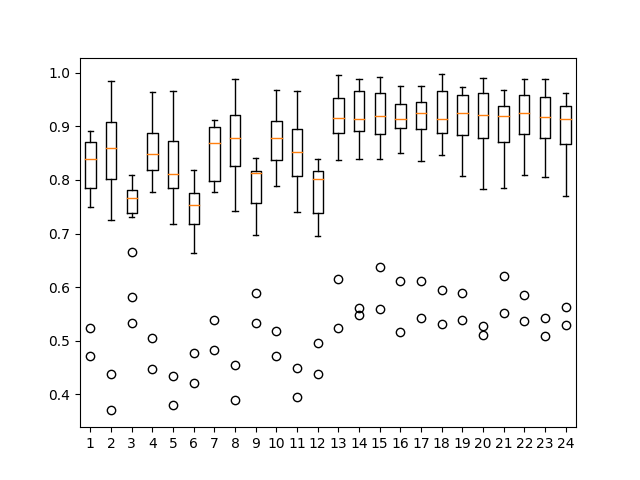
\includegraphics[scale=0.4]{acc_medium_all.png}}
	\subfigure[\emph{kappa} + reducción]{\label{fig:b}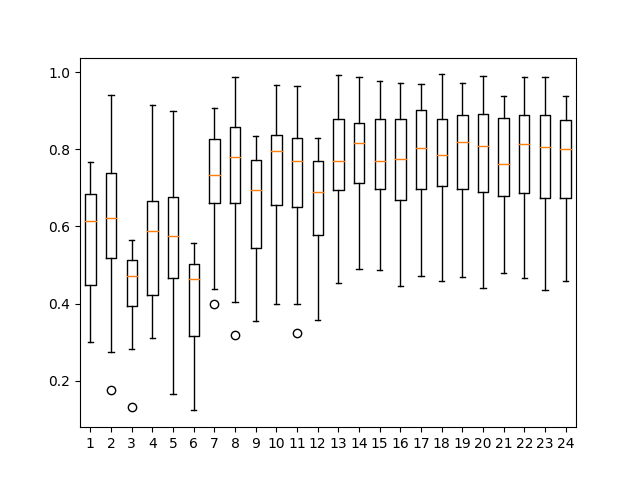
\includegraphics[scale=0.4]{kappa_medium_all.png}}

\caption{Boxplots de las variaciones de las metaheurísticas para los conjuntos medianos}
\label{medium-all}
\end{figure}

\begin{table}[h!]
\centering
\begin{tabular}{l c c c c c c}
\hline
\multirow{2}{*}{\textsc{Algoritmo}}
	& \multicolumn{2}{c}{\textsc{Accuracy}}
	& \multicolumn{2}{c}{\textsc{Kappa}}
	& \textsc{Reducción}
	& \textsc{Tiempo (seg)} \\
	& Training & Test
	& Training & Test \\ 
\hline
\hline

GGA         & 0.8702 & 0.7982 & 0.7375 & 0.5812 & 0.5641 & 110.0812 \\
\textbf{CNN-GGA}     & \textbf{0.7990} & \textbf{0.7051} & \textbf{0.5952} & \textbf{0.4426} & \textbf{0.7745} & \textbf{232.8342} \\
ENN-GGA     & 0.8475 & 0.8071 & 0.6949 & 0.5965 & 0.2862 & 125.8465 \\
RSS-GGA     & 0.8027 & 0.7520 & 0.5575 & 0.4547 & 0.6733 & 137.0381 \\
CNN-RSS-GGA & 0.8932 & 0.7890 & 0.7571 & 0.5516 & 0.5514 & 309.4603 \\
ENN-RSS-GGA & 0.9141 & 0.8155 & 0.8246 & 0.6168 & 0.1981 & 314.2968 \\

\hline

SSGA & 0.8431 & 0.8029 & 0.6676 & 0.5871 & 0.8392 & 3.5589 \\
CNN-SSGA & 0.8540 & 0.8007 & 0.6965 & 0.5923 & 0.8547 & 6.4410 \\
ENN-SSGA & 0.8200 & 0.8009 & 0.6324 & 0.5793 & 0.7459 & 5.6722 \\
\textbf{RSS-SSGA} & \textbf{0.8302} & \textbf{0.8045} & \textbf{0.6389} & \textbf{0.5854} & \textbf{0.8690} & \textbf{5.9946} \\
CNN-RSS-SSGA & 0.8586 & 0.8047 & 0.7043 & 0.5977 & 0.8121 & 10.5868 \\
ENN-RSS-SSGA & 0.8550 & 0.8078 & 0.7042 & 0.6004 & 0.7049 & 10.4293 \\

\hline

MA   & 0.8057 & 0.7908 & 0.5825 & 0.5564 & 0.9624 & 73.3461 \\
\textbf{CNN-MA} & \textbf{0.8116} & \textbf{0.8021} & \textbf{0.6000} & \textbf{0.5765} & \textbf{0.9572} & \textbf{57.3939} \\
ENN-MA & 0.7938 & 0.7925 & 0.5747 & 0.5608 & 0.9707 & 67.5310 \\
RSS-MA & 0.7924 & 0.7893 & 0.5611 & 0.5449 & 0.9671 & 69.5927 \\
CNN-RSS-MA & 0.8051 & 0.8015 & 0.5962 & 0.5808 & 0.9654 & 121.2220 \\
ENN-RSS-MA & 0.8070 & 0.7971 & 0.5886 & 0.8070 & 0.9633 & 112.0309 \\

\hline

\textbf{CHC} & \textbf{0.8313} & \textbf{0.8115} & \textbf{0.6347} & \textbf{0.5986} & \textbf{0.9455} & \textbf{2.8843} \\
CNN-CHC & 0.8303 & 0.8081 & 0.6337 & 0.5925 & 0.9352 & 4.6572 \\
ENN-CHC & 0.8107 & 0.8032 & 0.6084 & 0.5834 & 0.9356 & 5.0976 \\
RSS-CHC & 0.8151 & 0.8058 & 0.6074 & 0.5851 & 0.9535 & 4.7450 \\
CNN-RSS-CHC & 0.8276 & 0.8073 & 0.6280 & 0.5871 & 0.9319 & 6.7859 \\
ENN-RSS-CHC  & 0.8255 & 0.8074 & 0.6355 & 0.5944 & 0.9154 & 7.0284 \\


\hline
\end{tabular}
\caption{Promedios de las distintas variaciones de cada metaheurística para los conjuntos medianos}
\label{med-all}
\end{table}

\begin{table}[h!]
\centering
\begin{adjustbox}{max width =\textwidth}
\begin{tabular}{l c c c c c}
\hline
	\textsc{Algoritmo}
	& \multicolumn{1}{c}{\textsc{Accuracy}}
	& \multicolumn{1}{c}{\textsc{Kappa}}
	& \multicolumn{1}{c}{\textsc{Reducción}} 
	& \multicolumn{1}{c}{\textsc{Accuracy + reducción}} 
	& \multicolumn{1}{c}{\textsc{kappa + reducción}} \\
\hline
\hline

 & p-valor & p-valor & p-valor & p-valor & p-valor \\

CNN-GGA\\
vsGGA & 6.249e-04 & 1.116e-03 & 3.307e-03 & 1.260e-02 & 7.662e-02 \\ 
vsRSS-GGA & 1.001e-02 & 1.712e-01 & 1.758e-02 & 4.209e-01 & 1.842e-01 \\ 
vsCNN-RSS-GGA & 2.137e-04 & 2.137e-04 & 1.318e-04 & 9.673e-04 & 1.124e-02 \\
 
\hline

RSS-GGA\\
vsGGA & 1.001e-02 & 6.210e-03 & 2.543e-03 & 8.903e-03 & 8.092e-01 \\ 
vsCNN-RSS-GGA & 5.491e-03 & 7.231e-04 & 1.318e-04 & 2.137e-04 & 1.842e-01 \\

\hline

GGA\\
vsCNN-RSS-GGA & 6.210e-03 & 1.576e-02 & 7.475e-01 & 1.000e+00 & 4.209e-01 \\ 

\hline

\end{tabular}
\end{adjustbox}
\caption[Pruebas de \emph{Wilcoxon} entre GGA y variaciones para conjuntos medianos]{$p$-valor de pruebas de rangos con signo de \emph{Wilcoxon} para GGA sobre conjuntos medianos}
\label{wilcox-gga-med}
\end{table}

\begin{table}[h!]
\centering
\begin{adjustbox}{max width =\textwidth}
\begin{tabular}{l c c c c c}
\hline
	\textsc{Algoritmo}
	& \multicolumn{1}{c}{\textsc{Accuracy}}
	& \multicolumn{1}{c}{\textsc{Kappa}}
	& \multicolumn{1}{c}{\textsc{Reducción}} 
	& \multicolumn{1}{c}{\textsc{Accuracy + reducción}} 
	& \multicolumn{1}{c}{\textsc{kappa + reducción}} \\
\hline
\hline

 & p-valor & p-valor & p-valor & p-valor & p-valor \\

RSS-SSGA\\
vsSSGA & 4.326e-01 & 9.100e-02 & 4.274e-03 & 7.013e-03 & 5.857e-02 \\
vsCNN-SSGA & 4.093e-01 & 5.732e-01 & 3.760e-01 & 2.772e-01 & 6.874e-01 \\ 
vsCNN-RSS-SSGA & 9.039e-01 & 1.474e-01 & 1.318e-04 & 1.318e-04 & 6.249e-04 \\

\hline

SSGA\\
vsCNN-SSGA & 4.421e-02 & 2.196e-01 & 4.862e-02 & 1.712e-01 & 1.712e-01 \\  
vsCNN-RSS-SSGA & 3.341e-01 & 7.782e-01 & 1.909e-01 & 1.978e-01 & 2.598e-01 \\ 

\hline

CNN-SSGA\\
vsCNN-RSS-SSGA & 2.263e-03 & 3.858e-02 & 2.137e-04 & 4.634e-04 & 1.696e-03 \\


\hline

\end{tabular}
\end{adjustbox}
\caption[Pruebas de \emph{Wilcoxon} entre SSGA y variaciones para conjuntos medianos]{$p$-valor de pruebas de rangos con signo de \emph{Wilcoxon} para SSGA sobre conjuntos medianos}
\label{wilcox-SSGA-med}
\end{table}


\begin{table}[h!]
\centering
\begin{adjustbox}{max width =\textwidth}
\begin{tabular}{l c c c c c}
\hline
	\textsc{Algoritmo}
	& \multicolumn{1}{c}{\textsc{Accuracy}}
	& \multicolumn{1}{c}{\textsc{Kappa}}
	& \multicolumn{1}{c}{\textsc{Reducción}} 
	& \multicolumn{1}{c}{\textsc{Accuracy + reducción}} 
	& \multicolumn{1}{c}{\textsc{kappa + reducción}} \\

\hline
\hline

 & p-valor & p-valor & p-valor & p-valor & p-valor \\

MA\\
vsCNN-MA     & 3.760e-01 & 6.292e-01 & 4.688e-01 & 1.000e+00 & 7.782e-01 \\ 
vsENN-MA     & 5.066e-01 & 3.981e-01 & 3.958e-01 & 3.869e-01 & 3.271e-01 \\ 
vsRSS-MA     & 5.094e-02 & 4.862e-02 & 3.241e-01 & 4.688e-01 & 2.273e-01 \\ 
vsCNN-RSS-MA & 6.009e-01 & 4.209e-01 & 8.721e-01 & 6.874e-01 & 6.874e-01 \\ 
vsENN-RSS-MA & 8.446e-01 & 8.789e-01 & 9.679e-01 & 7.172e-01 & 9.359e-01 \\ 
 
\hline

CNN-MA\\
vsENN-MA & 8.789e-01 & 9.826e-01 & 2.954e-01 & 4.445e-01 & 4.445e-01 \\  
vsRSS-MA & 5.341e-02 & 1.075e-01 & 4.445e-01 & 4.939e-01 & 3.144e-01 \\ 
vsCNN-RSS-MA  & 9.679e-01 & 7.172e-01 & 7.782e-01 & 6.009e-01 & 5.732e-01 \\
vsENN-RSS-MA & 2.122e-01 & 4.445e-01 & 1.989e-01 & 9.039e-01 & 9.358e-01 \\

\hline

ENN-MA\\
vsRSS-MA  & 1.075e-01 & 1.712e-01 & 6.475e-01 & 2.954e-01 & 1.531e-01 \\ 
vsCNN-RSS-MA  & 3.547e-01 & 3.981e-01 & 3.981e-01 & 4.209e-01 & 6.580e-01 \\
vsENN-RSS-MA & 9.519e-01 & 8.092e-01 & 8.721e-01 & 8.721e-01 & 5.732e-01 \\ 

\hline

RSS-MA\\
vsCNN-RSS-MA & 7.908e-03 & 1.758e-02 & 1.842e-01 & 2.432e-01 & 7.662e-02 \\
vsENN-RSS-MA  & 7.662e-02 & 5.341e-02 & 4.939e-01 & 8.721e-01 & 5.461e-01 \\ 

\hline

CNN-RSS-MA\\
vsENN-RSS-MA  & 1.365e-01 & 2.122e-01 & 5.732e-01 & 1.842e-01 & 3.760e-01 \\ 

\hline

\end{tabular}
\end{adjustbox}
\caption[Pruebas de \emph{Wilcoxon} entre MA y variaciones para conjuntos medianos]{$p$-valor de pruebas de rangos con signo de \emph{Wilcoxon} para MA sobre conjuntos medianos}
\label{wilcox-MA-med}
\end{table}

\begin{table}[h!]
\centering
\begin{adjustbox}{max width =\textwidth}
\begin{tabular}{l c c c c c}
\hline
	\textsc{Algoritmo}
	& \multicolumn{1}{c}{\textsc{Accuracy}}
	& \multicolumn{1}{c}{\textsc{Kappa}}
	& \multicolumn{1}{c}{\textsc{Reducción}} 
	& \multicolumn{1}{c}{\textsc{Accuracy + reducción}} 
	& \multicolumn{1}{c}{\textsc{kappa + reducción}} \\

\hline
\hline

 & p-valor & p-valor & p-valor & p-valor & p-valor \\

CHC\\
vsCNN-CHC     & 5.817e-02 & 5.094e-02 & 8.248e-01 & 3.652e-01 & 1.262e-01 \\ 
vsENN-CHC     & 6.009e-01 & 8.092e-01 & 4.862e-02 & 2.977e-02 & 8.356e-02 \\ 
vsRSS-CHC     & 2.179e-02 & 1.124e-02 & 2.977e-02 & 9.679e-01 & 2.772e-01 \\ 
vsCNN-RSS-CHC & 2.977e-02 & 2.977e-02 & 2.422e-02 & 7.901e-03 & 1.000e-02 \\ 
vsENN-RSS-CHC & 2.351e-01 & 1.000e+00 & 2.134e-04 & 1.819e-04 & 8.375e-04 \\  

\hline

CNN-CHC\\
vsENN-CHC & 7.226e-01 & 4.074e-01 & 1.119e-01 & 1.590e-01 & 5.197e-01 \\
vsRSS-CHC & 6.579e-01 & 5.197e-01 & 1.227e-02 & 2.273e-01 & 2.432e-01 \\
vsCNN-RSS-CHC & 7.172e-01 & 5.066e-01 & 9.896e-02 & 6.707e-02 & 2.122e-01 \\ 
vsENN-RSS-CHC  & 6.292e-01 & 1.712e-01 & 2.977e-02 & 3.820e-02 & 4.860e-02 \\

\hline

ENN-CHC\\
vsRSS-CHC & 8.353e-02 & 2.688e-02 & 5.857e-02 & 3.292e-02 & 3.547e-01 \\
vsCNN-RSS-CHC & 2.860e-01 & 5.857e-02 & 4.445e-01 & 4.209e-01 & 6.009e-01 \\  
vsENN-RSS-CHC & 9.306e-01 & 9.133e-01 & 1.476e-03 & 1.576e-02 & 1.590e-01 \\ 

\hline

RSS-CHC\\
vsCNN-RSS-CHC & 7.475e-01 & 8.405e-01 & 3.411e-04 & 4.634e-04 & 2.688e-02 \\
vsENN-RSS-CHC & 4.565e-01 & 1.075e-01 & 1.316e-04 & 3.416e-04 & 1.758e-02 \\

\hline

CNN-RSS-CHC\\
vsENN-RSS-CHC  & 1.841e-01 & 6.415e-02 & 1.981e-02 & 5.857e-02 & 3.981e-01 \\

\hline


\end{tabular}
\end{adjustbox}
\caption[Pruebas de \emph{Wilcoxon} entre CHC y variaciones para conjuntos medianos]{$p$-valor de pruebas de rangos con signo de \emph{Wilcoxon} para CHC sobre conjuntos medianos}
\label{wilcox-CHC-med}
\end{table}


Los \emph{boxplots} que van desde el 1 al 6 de la figura \ref{medium-all} muestran que para los conjuntos medianos CNN-GGA tiene la mejor relación entre \emph{accuracy} + reducción. Al ver los p-valores de la tabla \ref{wilcox-gga-med} se tiene que CNN-GGA presenta valores similares RSS-GGA y GGA en \emph{accuracy} + reducción. Al revisar la tabla \ref{med-all} CNN-GGA es la variación que tiene la mejor tasa de reducción con 77.45\%.

Con respecto a \emph{kappa} + reducción, la figura \ref{medium-all} muestra un desempeño muy similar entre GGA, CNN-GGA, RSS-GGA y CNN-RSS-GGA. Al ver los p-valores de la tabla \ref{wilcox-gga-med} se obtiene que estos cuatro métodos son estadísticamente similares. La tabla \ref{med-all} muestra que GGA y CNN-RSS-GGA tienen un mayor nivel de \emph{kappa} que CNN-GGA y RSS-GGA, pero estos dos últimos compensan teniendo una reducción mayor.

Al comparar los tiempos, se tiene que ENN-GGA y RSS-GGA son las variantes más rápidas de GGA, con 15.76 y 26.95 segundos más de cómputo que GGA con inicialización aleatoria.

Para los conjuntos medianos CNN-GGA es la mejor opción entre las variaciones de GGA con 21.04\% más reducción que GGA.

Los \emph{boxplots} que comprenden desde el 6 al 12 de la figura \ref{medium-all} muestran que SSGA, CNN-SSGA, RSS-SSGA y CNN-RSS-SSGA son muy similares entre sí para \emph{accuracy} + reducción y \emph{kappa} + reducción. Los p-valores de la tabla \ref{wilcox-SSGA-med} muestran que la única diferencia se da en \emph{accuracy} + reducción entre SSGA y RSS-SSGA, de resto las cuatro variaciones son estadísticamente similares en \emph{kappa} + reducción. La tabla \ref{med-all} muestra valores muy parejos en \emph{accuracy, kappa} y reducción. En este caso, RSS-SSGA destaca del resto por presentar ĺa tasa reducción más alta con 86.90\%, que es 1.43\% mayor a la tasa de reducción de CNN-SSGA y es 2.98\% mayor que la tasa de reducción de SSGA.

En tiempo de cómputo se tiene que ENN-SSGA y RSS-SSGA son las variaciones más rápidas, con 2.12 y 2.44 segundos más que SSGA.

RSS-SSGA es entonces, la mejor opción entre las variantes de SSGA para los conjuntos medianos, con 2.98\% más reducción que SSGA y a cambio de 2.44 segundos más de tiempo de cómputo.

Los \emph{boxplots} que van desde el 13 al 18 de la figura \ref{medium-all} muestran valores muy similares entre todas las variaciones de MA para \emph{accuracy} + reducción y para \emph{kappa} + reducción. Ninguna variante destaca sobre otra, la tabla \ref{wilcox-MA-med} confirma que todas las variaciones son estadísticamente similares, además, la tabla  \ref{med-all}  no muestra una diferencia real entre las variaciones.

En relación al tiempo de cómputo, CNN-MA es la variación más rápida de todas, siendo más rápido que MA por 15.95 segundos en promedio. Esto se debe a que utilizando CNN, MA tiene menos llamadas al proceso de optimización interna que con una población inicial aleatoria.

Por el tiempo de cómputo, se puede referir a CNN-MA como la mejor elección entre las distintas variantes de MA al momento de ser utilizado para conjuntos medianos.

Los \emph{boxplots} que van desde el 19 al 24 de la figura \ref{medium-all} muestran un comportamiento similar para todas las variantes de CHC, en donde todas presentan valores similares en \emph{accuracy} + reducción y \emph{kappa} + reducción. Los p-valores de la tabla \ref{wilcox-CHC-med} muestra que CHC, CNN-CHC, ENN-CHC y RSS-CHC son estadísticamente similares. Los promedios de la tabla \ref{med-all} corroboran que CHC, CNN-CHC, ENN-CHC y RSS-CHC poseen valores similares.

De entre las cuatro variantes mencionadas anteriormente, se elige CHC con inicialización aleatoria como mejor versión de CHC ya que presenta los menores tiempos de cómputo, con un promedio de 2.88 segundos.

\begin{table}[h!]
\centering
\begin{adjustbox}{max width =\textwidth}
\begin{tabular}{l c c c c c}
\hline
	\textsc{Algoritmo}
	& \multicolumn{1}{c}{\textsc{Accuracy}}
	& \multicolumn{1}{c}{\textsc{Kappa}}
	& \multicolumn{1}{c}{\textsc{Reducción}} 
	& \multicolumn{1}{c}{\textsc{Accuracy + reducción}} 
	& \multicolumn{1}{c}{\textsc{kappa + reducción}} \\

\hline
\hline

CNN-GGA\\
vsRSS-SSGA & 2.502e-04 & 6.249e-04 & 1.410e-02 & 2.137e-04 & 2.137e-04 \\ 
vsCNN-MA   & 2.502e-04 & 8.375e-04 & 1.822e-04 & 1.318e-04 & 1.318e-04 \\
vsCHC      & 2.137e-04 & 3.416e-04 & 2.137e-04 & 1.318e-04 & 1.318e-04 \\

\hline

RSS-SSGA\\
vsCNN-MA & 8.092e-01 & 7.475e-01 & 1.316e-04 & 1.318e-04 & 2.134e-04 \\
vsCHC    & 1.576e-02 & 8.903e-03 & 1.551e-04 & 1.318e-04 & 1.318e-04 \\

\hline

CNN-MA\\
vsCHC & 3.820e-02 & 1.260e-02 & 1.365e-01 & 6.292e-01 & 5.197e-01 \\

\hline

\end{tabular}
\end{adjustbox}
\caption[Pruebas de \emph{Wilcoxon} entre las mejores variaciones de cada metaheurística para conjuntos medianos]{$p$-valor de pruebas de rangos con signo de \emph{Wilcoxon} para las mejores variantes de las metaheurísticas sobre conjuntos medianos}
\label{wilcox-best-med}
\end{table}

\begin{table}[h!]
\centering
\begin{adjustbox}{max width =\textwidth}
\begin{tabular}{l c c|l c c|l c c}
\hline
\multicolumn{3}{c|}{\textsc{Accuracy + Reducción}}
	& \multicolumn{3}{c|}{\textsc{Kappa + Reducción}}
	& \multicolumn{3}{c}{\textsc{Tiempo}} \\
\hline
Algoritmo & Rank & Mejor & Algoritmo & Rank & Mejor & Algoritmo & Rank & Mejor \\
\hline
\hline

CNN-RSS-MA   & 4.76  & 5 & CHC          & 5.05  & 2  &  CHC          & 1.41 & 13 \\
ENN-MA       & 5.05  & 4 & ENN-MA       & 5.41  & 4  &  SSGA         & 1.94 & 3 \\
CHC          & 5.52  & 2 & CNN-RSS-MA   & 5.52  & 5  &  CNN-CHC      & 4.11 & 0 \\
CNN-MA       & 5.94  & 3 & RSS-CHC      & 6.52  & 0  &  RSS-CHC      & 4.58 & 0 \\
ENN-RSS-MA   & 5.94  & 1 & CNN-MA       & 6.76  & 2  &  ENN-CHC      & 5.00 & 0 \\
RSS-CHC      & 5.94  & 0 & ENN-RSS-MA   & 7.05  & 1  &  ENN-SSGA     & 5.52 & 0 \\
MA           & 6.29  & 0 & MA           & 7.23  & 1  &  RSS-SSGA     & 7.17 & 0 \\
RSS-MA       & 7.05  & 1 & CNN-CHC      & 7.23  & 0  &  CNN-SSGA     & 7.36 & 1 \\
CNN-CHC      & 7.35  & 0 & ENN-CHC      & 7.47  & 1  &  ENN-RSS-CHC  & 9.05 & 0 \\
ENN-CHC      & 8.41  & 0 & CNN-RSS-CHC  & 8.29  & 0  &  CNN-RSS-CHC  & 9.11 & 0 \\
CNN-RSS-CHC  & 8.70  & 0 & RSS-MA       & 8.41  & 0  &  ENN-RSS-SSGA & 11.23 & 0 \\
ENN-RSS-CHC  & 10.00 & 1 & ENN-RSS-CHC  & 8.47  & 1  &  CNN-RSS-SSGA & 11.47 & 0 \\
RSS-SSGA     & 13.47 & 0 & CNN-SSGA     & 12.94 & 0  &  MA           & 14.35 & 0 \\
CNN-SSGA     & 13.47 & 0 & RSS-SSGA     & 13.05 & 0  &  RSS-MA       & 14.64 & 0 \\
SSGA         & 14.70 & 0 & SSGA         & 14.23 & 0  &  CNN-MA       & 15.23 & 0 \\
CNN-RSS-SSGA & 15.82 & 0 & CNN-RSS-SSGA & 15.05 & 0  &  ENN-MA       & 15.23 & 0 \\
ENN-SSGA     & 16.64 & 0 & ENN-SSGA     & 16.76 & 0  &  CNN-RSS-MA   & 17.88 & 0 \\
CNN-GGA      & 18.17 & 0 & ENN-RSS-SSGA & 18.00 & 0  &  ENN-RSS-MA   & 18.23 & 0 \\
ENN-RSS-SSGA & 18.47 & 0 & CNN-GGA      & 18.52 & 0  &  GGA          & 18.88 & 0 \\
RSS-GGA      & 19.94 & 0 & GGA          & 20.47 & 0  &  ENN-GGA      & 19.52 & 0 \\
GGA          & 21.00 & 0 & RSS-GGA      & 20.52 & 0  &  RSS-GGA      & 20.05 & 0 \\
CNN-RSS-GGA  & 21.41 & 0 & CNN-RSS-GGA  & 21.23 & 0  &  CNN-GGA      & 21.76 & 0 \\
ENN-GGA      & 22.05 & 0 & ENN-GGA      & 22.05 & 0  &  ENN-RSS-GGA  & 22.76 & 0 \\
ENN-RSS-GGA  & 23.82 & 0 & ENN-RSS-GGA  & 23.64 & 0  &  CNN-RSS-GGA  & 23.41 & 0 \\ 

\hline
\end{tabular}
\end{adjustbox}
\caption{Rangos de las metaheurísticas en \emph{accuracy + reducción}, \emph{kappa + reducción} y tiempo para los conjuntos medianos}
\label{rank-med}
\end{table}

Teniendo las mejores variaciones de cada metaheurística para los conjuntos medianos: CNN-GGA, RSS-SSGA, CNN-MA y CHC, se hace una comparación entre ellos para determinar cuál es la mejor opción. La figura \ref{medium-all} muestra que '14':CNN-MA y '19':CHC presentan los mejores valores en \emph{accuracy} + reducción y \emph{kappa} + reducción. La tabla \ref{wilcox-best-med} muestra que CNN-MA y CHC son estadísticamente similares y esto se puede apreciar al comparar los valores de la tabla \ref{med-all}. 

En la tabla \ref{rank-med} las variaciones de MA y CHC comparten los primeros puestos al tener los mejores valores en \emph{accuracy, kappa} y reducción. La diferencia principal entre ambas vuelve a estar en el tiempo de cómputo, el cual hace a CHC con inicialización aleatoria la mejor opción a elegir para los conjuntos medianos, ya que tarda 54.51 segundos menos que CNN-MA en devolver un resultado.


\paragraph{Conjuntos Grandes}

\begin{table}[h!]
\centering
\begin{tabular}{l c c c c c c}
\hline
\multirow{2}{*}{\textsc{Algoritmo}}
	& \multicolumn{2}{c}{\textsc{Accuracy}}
	& \multicolumn{2}{c}{\textsc{Kappa}}
	& \textsc{Reducción}
	& \textsc{Tiempo (seg)} \\
	& Training & Test
	& Training & Test \\ 
\hline
\hline

GGA         & 0.9316 & 0.8644 & 0.7994 & 0.6014 & 0.5050 & 672.0273 \\
CNN-GGA     & 0.7106 & 0.6431 & 0.4478 & 0.3094 & 0.8409 & 1568.8913 \\
ENN-GGA     & 0.9357 & 0.8890 & 0.7944 & 0.6453 & 0.1502 & 718.0400 \\
\textbf{RSS-GGA}     & \textbf{0.9150} & \textbf{0.8719} & \textbf{0.7227} & \textbf{0.5821} & \textbf{0.7083} & \textbf{1197.0505} \\
CNN-RSS-GGA & 0.9455 & 0.8588 & 0.8410 & 0.5885 & 0.6089 & 2646.6438 \\
ENN-RSS-GGA & 0.9574 & 0.9574 & 0.9574 & 0.6238 & 0.1025 & 1703.4263 \\

\hline

SSGA & 0.8911 & 0.8743 & 0.6953 & 0.6201 & 0.8056 & 27.6637 \\
CNN-SSGA & 0.8897 & 0.8512 & 0.7002 & 0.5939 & 0.8807 & 90.1004 \\
ENN-SSGA & 0.9097 & 0.8892 & 0.7113 & 0.6441 & 0.6823 & 34.9024 \\
\textbf{RSS-SSGA} & \textbf{0.8968} & \textbf{0.8826} & \textbf{0.6743} & \textbf{0.6271} & \textbf{0.8927} & \textbf{57.7995} \\
CNN-RSS-SSGA & 0.9002 & 0.8634 & 0.7140 & 0.6069 & 0.8434 & 99.1629 \\
ENN-RSS-SSGA & 0.9112 & 0.8805 & 0.7245 & 0.6272 & 0.6668 & 78.5967 \\

\hline

\textbf{MA}   & \textbf{0.8904} & \textbf{0.8999} & \textbf{0.6499} & \textbf{0.6510} & \textbf{0.9973} & \textbf{256.1432} \\
CNN-MA & 0.8925 & 0.8926 & 0.6360 & 0.6341 & 0.9884 & 612.7902 \\
ENN-MA & 0.8807 & 0.8902 & 0.6072 & 0.6145 & 0.9976 & 288.6525 \\
RSS-MA & 0.9000 & 0.9002 & 0.6347 & 0.6343 & 0.9746 & 527.9115 \\
CNN-RSS-MA & 0.8857 & 0.8951 & 0.6176 & 0.6160 & 0.9707 & 960.3951 \\
ENN-RSS-MA & 0.8746 & 0.8912 & 0.6292 & 0.6386 & 0.9969 & 443.0003 \\

\hline

\textbf{CHC}  & \textbf{0.8961} & \textbf{0.8934} & \textbf{0.6614} & \textbf{0.6506} & \textbf{0.9615} & \textbf{16.8665} \\
CNN-CHC & 0.8903 & 0.8871 & 0.6554 & 0.6437 & 0.9771 & 38.3314 \\
ENN-CHC & 0.8993 & 0.8964 & 0.6746 & 0.6631 & 0.9233 & 27.3520 \\
RSS-CHC & 0.8972 & 0.8962 & 0.6591 & 0.6526 & 0.9819 & 41.1142 \\
CNN-RSS-CHC & 0.8945 & 0.8910 & 0.8945 & 0.6435 & 0.9719 & 50.5800 \\
ENN-RSS-CHC & 0.8975 & 0.8922 & 0.6721 & 0.6532 & 0.9099 & 47.4006 \\

\hline
\end{tabular}
\caption{Promedios de las distintas variaciones de cada metaheurística para los conjuntos grandes}
\label{grande-all}
\end{table}

La tabla \ref{grande-all} muestra que RSS-GGA tiene la mejor relación en \emph{accuracy} + reducción, seguido por CNN-GGA, el cual tiene la mejor reducción. Para \emph{kappa} + reducción RSS-GGA, GGA y CNN-GGA se encuentran más parejos, estando RSS-GGA ligeramente por encima. En relación al tiempo, ENN-GGA es la variante más rápida, tardando 46.02 segundos más que GGA; mientras que RSS-GGA es la segunda variante más rápida, tardando 525.03 segundos más que GGA. Bajo estas consideraciones RSS-GGA es la mejor elección entre las variantes de GGA para los conjuntos grandes.

Para los conjuntos grandes, la tabla \ref{grande-all} revela que RSS-SSGA presenta la mejor relación entre \emph{accuracy, kappa} y reducción con 88.26\%, 62.71\% y 89.27\% respectivamente. Con respecto al tiempo, ENN-SSGA y RSS-SSGA son las variantes más rápidas, tardando 7.24 y 30.13 segundos más que SSGA respectivamente. Por estas razones, RSS-SSGA es la mejor elección entre las variantes de SSGA para los conjuntos grandes.

Con respecto a MA, la tabla \ref{grande-all} no muestra diferencias reales en \emph{accuracy, kappa} ni reducción entre las distintas variantes. En cambio, cuando se toma en cuenta el tiempo MA con inicialización aletaoria es la versión que tarda menos en devolver un resultado. Por lo tanto MA es la mejor opción para los conjuntos grandes.

Pasando a CH, la tabla \ref{grande-all} muestra valores muy similares en \emph{accuracy, kappa} y reducción para CHC, CNN-CHC, RSS-CHC y CNN-RSS-CHC. Es por eso que se decide cuál es la mejor opción a partir del tiempo de cómputo, siendo CHC con inicialización aleatoria la opción elegida para los conjuntos grandes.

Al comparar las mejores variantes de cada metaheurística: RSS-GGA, RSS-SSGA, MA y CHC; se tiene que MA con inicialización aleatoria es la metaheurística que presenta los mejores valores, teniendo un \emph{accuracy y kappa} similares a CHC y la mayor tasa de reducción con un 99.73\%, el cual es 3.58\% mayor que CHC. Por lo tanto, la mejor opción entre todas las variantes de metaheurísticas para los conjuntos grandes es MA. 

